\documentclass[svgnames,11pt]{beamer}
\input{/home/tof/Documents/Cozy/latex-include/preambule_commun.tex}
\input{/home/tof/Documents/Cozy/latex-include/preambule_beamer.tex}
%\usepackage{pgfpages} \setbeameroption{show notes on second screen=left}
\author[]{Christophe Viroulaud}
\title{Routing Information Protocol}
\date{\framebox{\textbf{Archi 11}}}
%\logo{}
\institute{Terminale - NSI}

\begin{document}
\begin{frame}
\titlepage
\end{frame}
\begin{frame}
    \frametitle{}

    \begin{center}
    \centering
    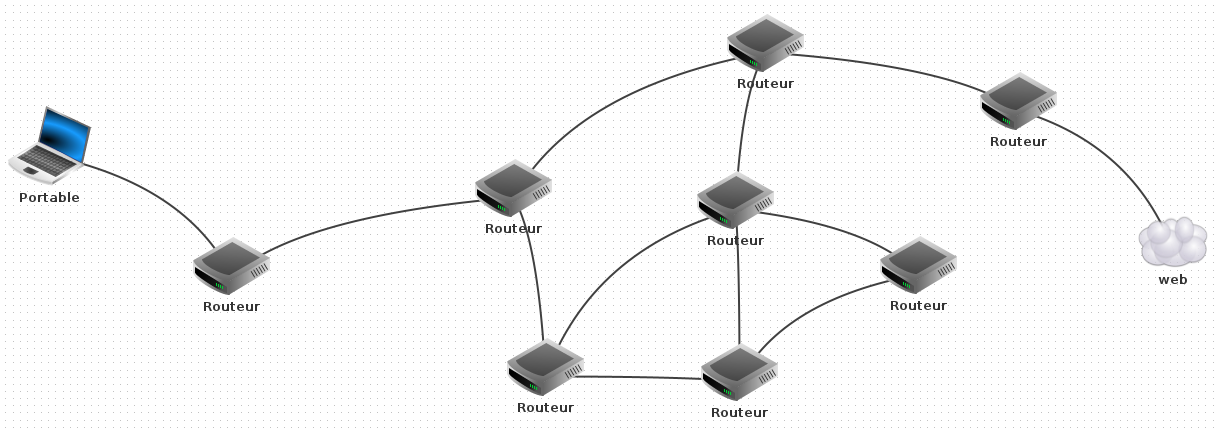
\includegraphics[width=8cm]{ressources/reseau-intro.png}
    \captionof{figure}{Les paquets d'informations se déplacent de routeurs en routeurs.}
    \label{IMG}
    \end{center}

\end{frame}
\begin{frame}
    \frametitle{}

\begin{framed}
    \centering Comment un routeur détermine la route à choisir?
\end{framed}
\end{frame}
\section{Protocole de routage}
\subsection{Principe}
\begin{frame}
    \frametitle{Protocole de routage - principe}
    En plus des paquets, les routeurs s’échangent des informations sur la topologie du réseau.
    \begin{aretenir}[]
        Chaque routeur applique les mêmes règles de communication et de description : c’est le protocole de routage.
    \end{aretenir}

\end{frame}
\subsection{Routing Information Protocol}
\begin{frame}
    \frametitle{Routing Information Protocol}

    À intervalle régulier (30 secondes par défaut), chaque routeur transmet à ses voisins:
    \begin{itemize}
        \item<1-> les adresses de ses propres voisins,
        \item<2-> celles qu’il a reçues par d’autres routeurs.
        \item<3-> Il précise également la distance (en
        nombre de sauts) pour atteindre une machine donnée.
    \end{itemize}

\end{frame}
\begin{frame}
    \frametitle{}

    \begin{aretenir}[]
        Le protocole RIP échange des vecteurs de distance (couple adresse/distance) avec ses routeurs voisins. L’objectif du protocole RIP est de minimiser le nombre de sauts pour atteindre la destination.
    \end{aretenir}

\end{frame}
\section{Table de routage}
\subsection{Rôle}
\begin{frame}
    \frametitle{Table de routage - rôle}
\begin{center}
        Chaque routeur construit une table de routage. Elle contient les informations des routes à suivre pour atteindre les autres réseaux.
\end{center}
    

\end{frame}
\begin{frame}
    \frametitle{}

    Chaque ligne de la table de routage contient quatre informations:
\begin{itemize}
    \item<1-> la \emph{destination} sous la forme adresse de sous-réseau/masque,
    \item<2-> la \emph{passerelle} est l'adresse IP du prochain routeur à traverser,
    \item<3-> l'\emph{interface} réseau à utiliser pour rejoindre la passerelle,
    \item<4-> la \emph{distance} vers la destination.
\end{itemize}

\end{frame}
\subsection{Construction}
\begin{frame}
    \frametitle{Construction}

    \begin{center}
    \centering
    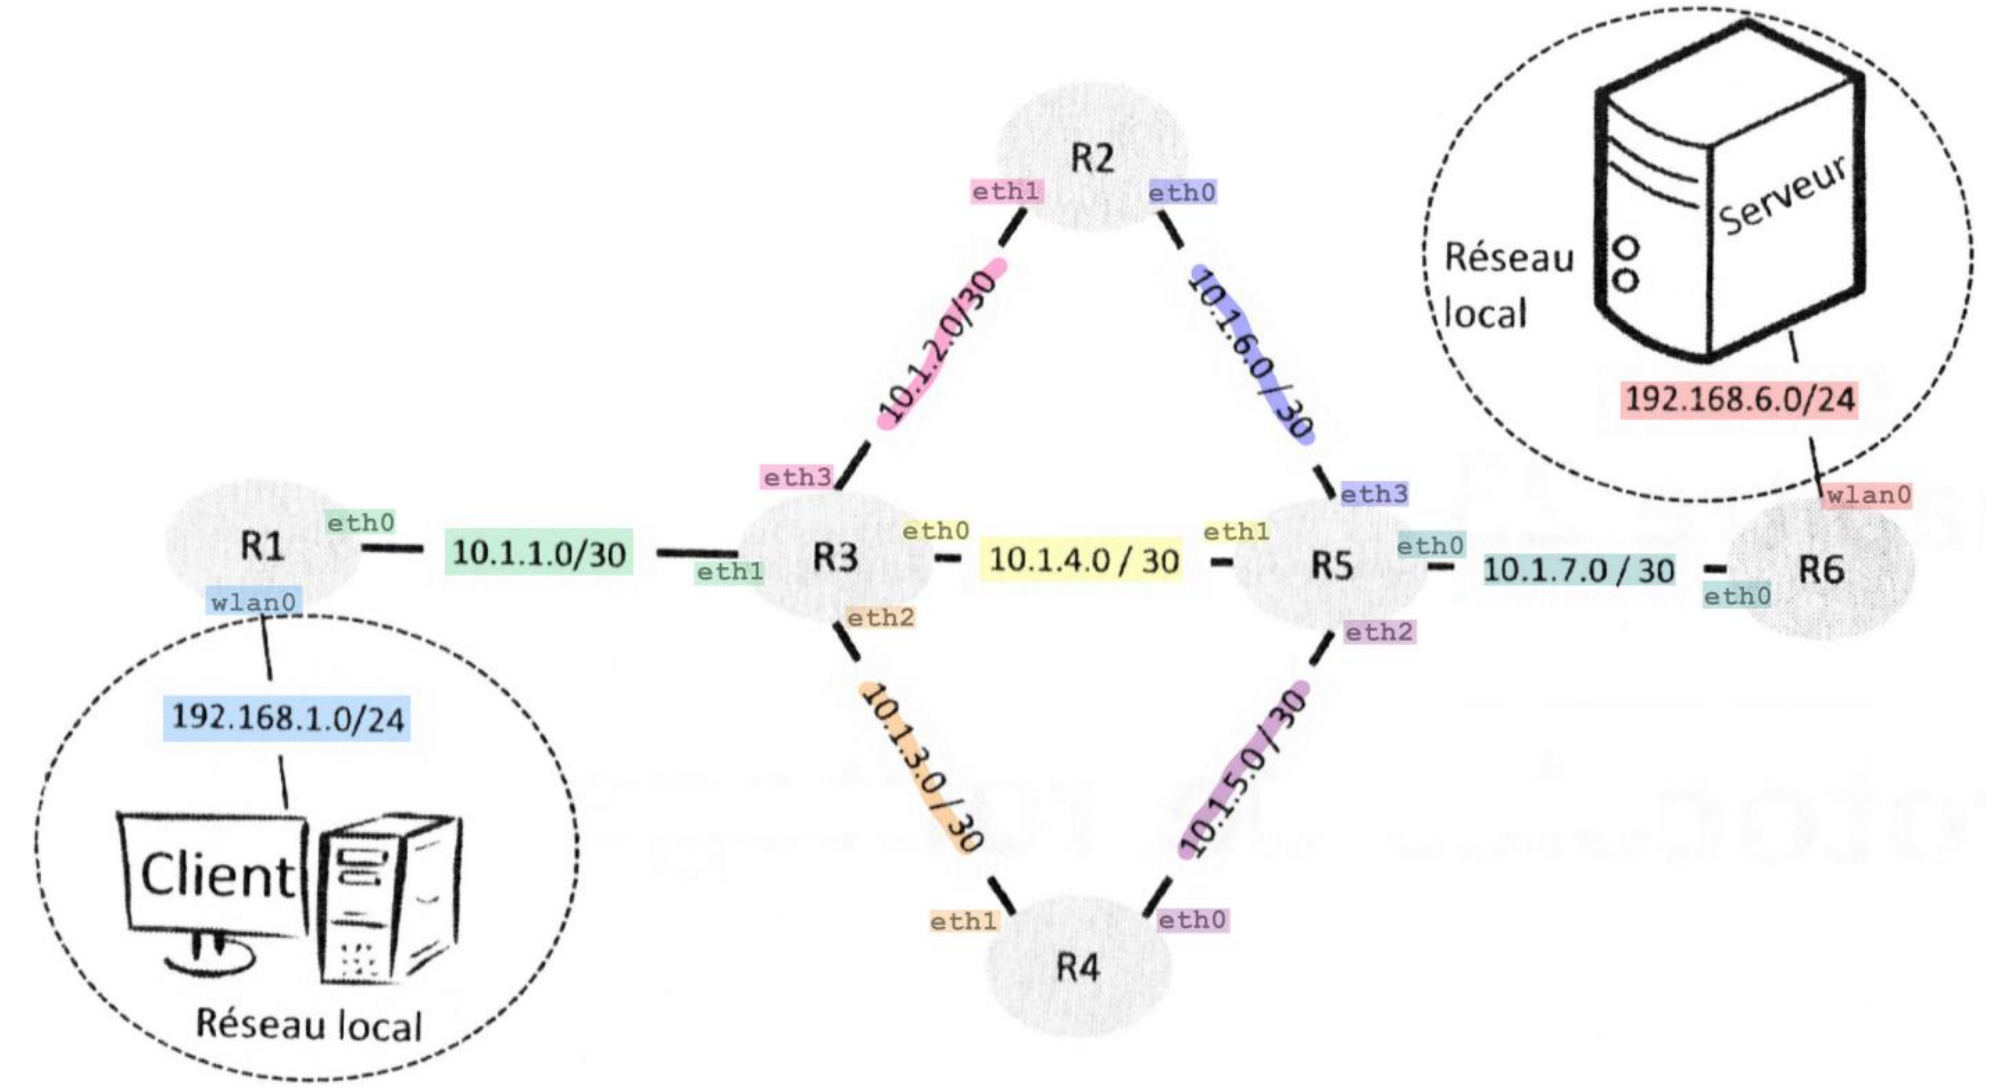
\includegraphics[width=10cm]{ressources/reseau.png}
    \captionof{figure}{Topologie d'un réseau}
    \label{IMG}
    \end{center}

\end{frame}

\begin{frame}
    \frametitle{Phase d'initialisation}
        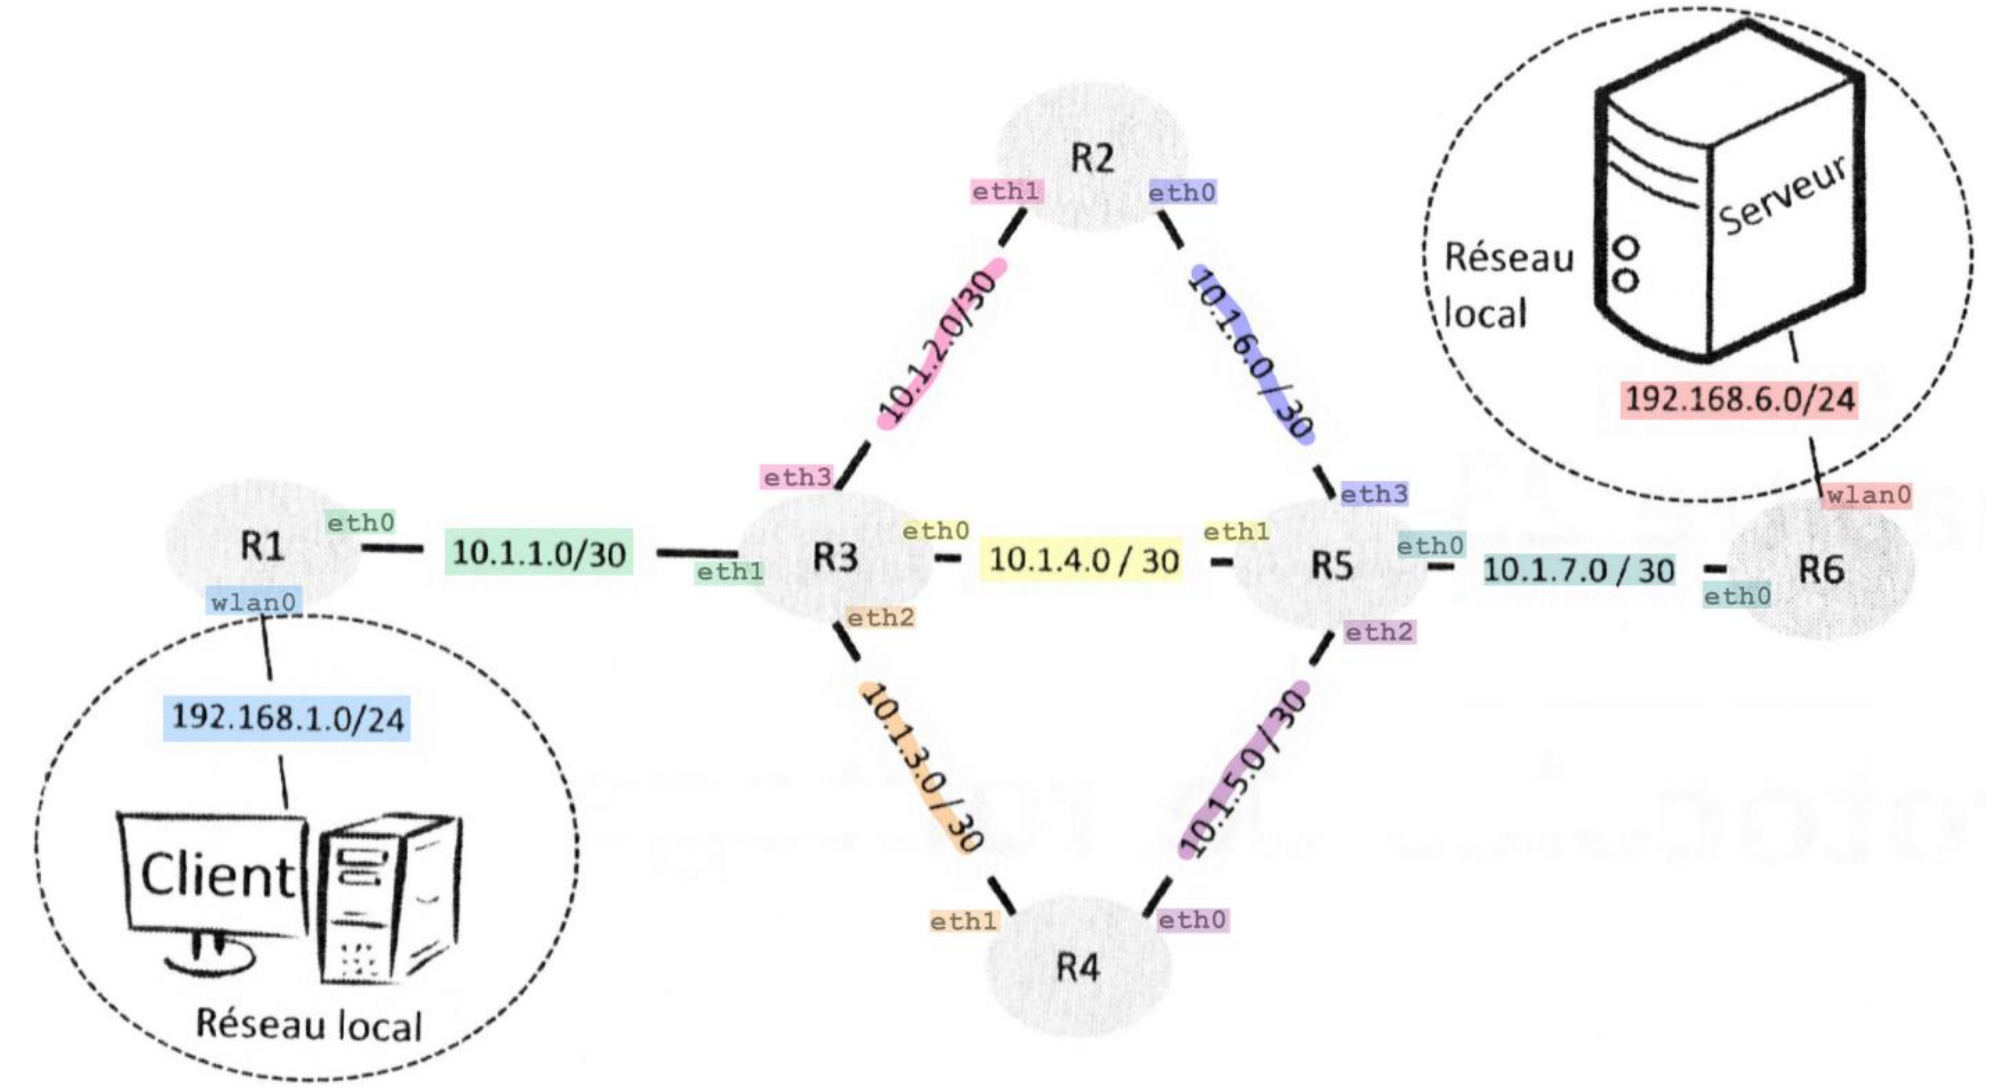
\includegraphics[width=9cm]{ressources/reseau.png}
\textbf{Phase d'initialisation (démarrage):} Le routeur récupère les informations de ses voisins immédiats.

        \begin{center}
    \begin{tabular}{|*{4}{c|}}
        \hline
        destination    & passerelle & interface & distance \\
        \hline
        10.1.1.0/30    &            & eth0      & 1        \\
        \hline
        192.168.1.0/24 &            & wlan0     & 1        \\
        \hline
    \end{tabular}
    \captionof{table}{Table de routage de R1}
\end{center}
\note{On atteint des réseaux (pas des routeurs) $\rightarrow$ passerelle vide pour les réseaux voisins.}
\end{frame}

\begin{frame}
    \frametitle{}
    \begin{center}
        \centering
        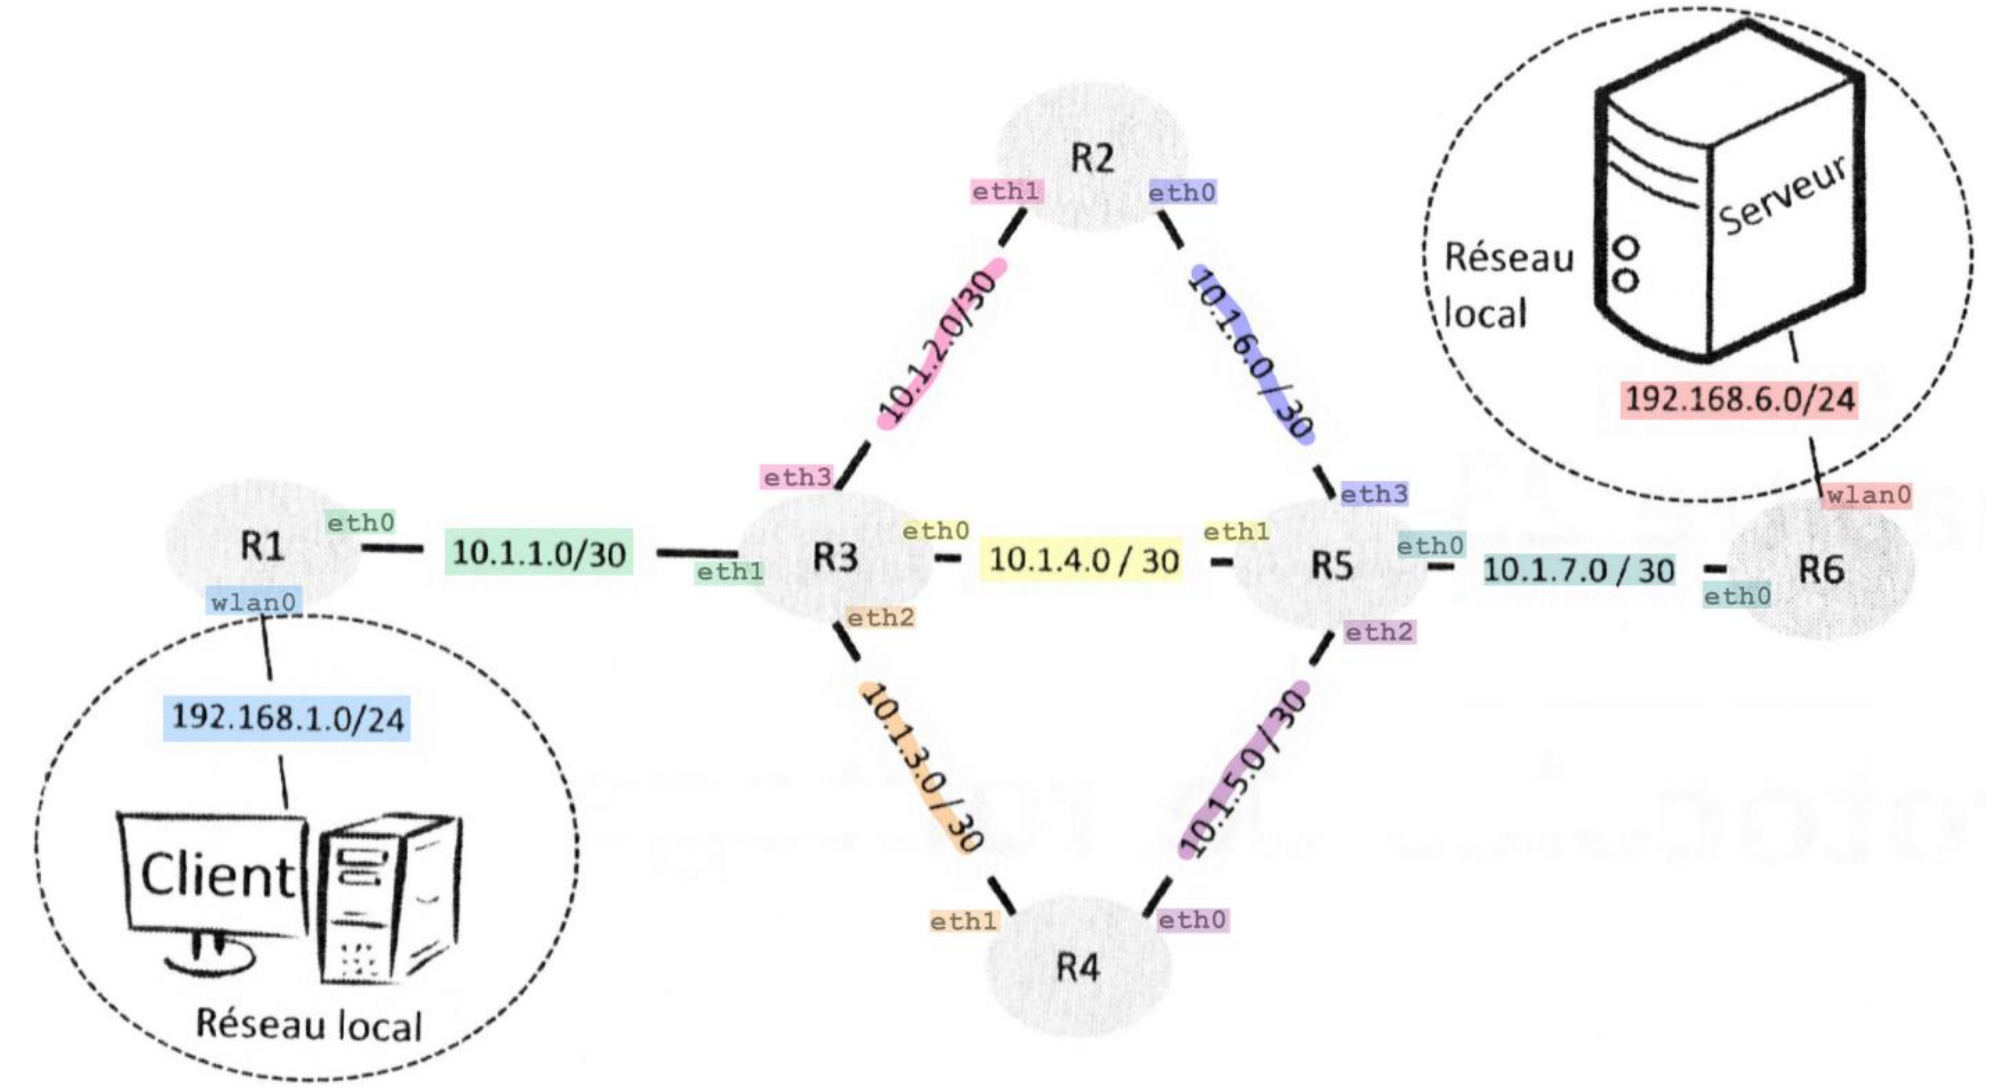
\includegraphics[width=10cm]{ressources/reseau.png}
        \captionof{figure}{Topologie du réseau}
        \label{reseau}
    \end{center}
    \begin{activite}
        Construire la table de routage du routeur R3 lors de la phase d'initialisation.
    \end{activite}

\end{frame}

\begin{frame}
    \frametitle{Correction}

    \begin{center}
        \begin{tabular}{|*{4}{c|}}
            \hline
            destination    & passerelle & interface & distance \\
            \hline
            10.1.1.0/30    &            & eth1      & 1        \\
            \hline
            10.1.2.0/30    &            & eth3      & 1        \\
            \hline
            10.1.3.0/30    &            & eth2      & 1        \\
            \hline
            10.1.4.0/30    &            & eth0      & 1        \\
            \hline
        \end{tabular}
        \captionof{table}{Table de routage de R3}
    \end{center}

\end{frame}
\end{document}